

\documentclass{article}
\usepackage{graphicx} % Required for inserting images
\usepackage[absolute,overlay]{textpos}
\setlength{\parindent}{0pt}
\usepackage{geometry}
\geometry{top=1in, bottom=1in, right=1in, left=1in}
\usepackage{multicol}
\usepackage{multirow}
\usepackage[pages=some]{background}

\usepackage{listings}
\usepackage{xcolor}
\usepackage{listings}

% Define C code style
\lstdefinestyle{CStyle}{
    language=C,
    basicstyle=\ttfamily\small,
    keywordstyle=\color{blue}\bfseries,
    stringstyle=\color{red},
    commentstyle=\color{green!50!black},
    numbers=left,
    numberstyle=\tiny\color{gray},
    stepnumber=1,
    numbersep=8pt,
    tabsize=4,
    showstringspaces=false,
    breaklines=true,
    frame=single
}

\pagestyle{empty}

\backgroundsetup{
  scale=1,
  opacity=1,
  angle=0,
  contents={
\includegraphics[width=\paperwidth,height=\paperheight]{imagenes/portada.jpg}}
}

\usepackage{xcolor}
\definecolor{rojo}{rgb}{0.8, 0, 0}

\usepackage{titlesec}


\titleformat{\section}
  {\color{rojo}\Large\bfseries}
  {}
  {0pt}
  {}

\titleformat{\subsection}
  {\color{rojo}\large\bfseries}
  {}
  {0pt}
  {}

\begin{document}
\BgThispage
\-
\begin{textblock*}{15cm}(4cm, 9cm)
    {\fontsize{30pt}{16pt}\selectfont
    \textcolor{rojo}{\textbf{REPORTE DE PRÁCTICA NO. 6}}
    }
\end{textblock*}
\begin{textblock*}{15cm}(4cm, 11cm)
    {\fontsize{15pt}{16pt}\selectfont
    \textcolor{rojo}{\textbf{NOMBRE DE LA PRÁCTICA: Análisis sintáctico de expresiones aritméticas}}
    }
\end{textblock*}
\begin{textblock*}{15cm}(6cm, 12.5cm)
    {\fontsize{13pt}{16pt}\selectfont
    \textcolor{rojo}{\textbf{ALUMNOS: Garcia Colmenares Andres \\ Arana Juarez Raul \\ Flores Guzman Oliver Alain \\}}
    }
\end{textblock*}
\begin{textblock*}{15cm}(9cm, 14.5cm)
    {\fontsize{11pt}{16pt}\selectfont
    \textcolor{rojo}{\textbf{Dr. Eduardo Cornejo-Velázquez}}
    }
\end{textblock*}

\newpage

\section{1. Introducción}
\textbf{Sintaxis y Gramáticas en los Lenguajes de Programación}

Todo lenguaje de programación está regido por un conjunto de reglas que determinan la estructura sintáctica 
de los programas bien formados. La descripción de la sintaxis de estas construcciones puede realizarse 
mediante Gramáticas Libres de Contexto o utilizando la Notación BNF (Backus-Naur Form). Estas opciones 
ofrecen ventajas para los diseñadores de lenguajes, así como a los desarrolladores de compiladores, ya que 
constituyen especificaciones sintácticas claras y precisas. 
 \\
Una gramática permite la generación automática de analizadores sintácticos, contribuyendo a la detección de 
ambigüedades durante el proceso de construcción. Al proporcionar una estructura formal al lenguaje de 
programación, facilita la generación de código y la identificación de errores. Además, la descripción de un 
lenguaje mediante una gramática simplifica su ampliación o modificación futura.
donde: \\

\textbf{Analizador Sintactico}

El analizador sintáctico constituye una etapa esencial en el proceso de compilación, encargándose de verificar 
que el texto de entrada cumpla con las reglas definidas por la gramática correspondiente. Si el programa de 
entrada es válido, el analizador genera un árbol sintáctico que representa su estructura. En teoría, la salida 
del analizador consiste en una representación formal del árbol sintáctico basada en la secuencia de tokens 
proporcionada por el analizador léxico. 
 
En la práctica, el analizador sintáctico suele realizar tareas adicionales, como: 
\begin{itemize}
\item  Acceso a la tabla de símbolos para asistir en las funciones del analizador semántico. 
\item  Verificación de tipos, propia del análisis semántico. 
\item  Generación de código intermedio. 
\item  Manejo y generación de mensajes de error. 
\end{itemize}

\textbf{Manejo de Errores Sintácticos} \\
 
El diseño de un compilador sería significativamente más sencillo si solo tuviera que procesar programas 
correctos. Sin embargo, en la práctica, los programadores suelen cometer errores, por lo que un buen 
compilador debe ser capaz de identificar, localizar y comunicar estos errores de manera efectiva. Incorporar 
estrategias de manejo de errores desde las etapas iniciales del desarrollo de un compilador no solo simplifica 
su estructura, sino que también mejora su capacidad para responder a los errores detectados.

Los errores que pueden surgir durante el proceso de programación incluyen: 
\begin{itemize}
\item Errores léxicos. Escribir incorrectamente un identificador, palabra clave u operador. 
\item Errores sintácticos. Derivados de expresiones mal formadas, como paréntesis desbalanceados o 
operadores mal ubicados. 
\item Errores semánticos. Aplicar un operador a un operando incompatible. 
\item Errores lógicos. Códigos con funciones recursivas infinitas. 
\end{itemize}
    \newpage

El manejo de errores sintácticos es especialmente complejo en la creación de compiladores. Un buen 
analizador sintáctico debe cumplir con los siguientes objetivos: 
\begin{itemize}
\item Reportar los errores de forma clara y precisa. 
\item Especificar el tipo de error y su ubicación. 
\item Recuperarse del error para continuar con el análisis del programa. 
\item Minimizar el impacto en el rendimiento de la compilación. 
\end{itemize}
Por lo tanto, un compilador robusto debe diseñarse considerando los errores potenciales, lo que no solo mejora 
su funcionalidad, sino que también garantiza una respuesta más eficiente ante los errores detectados. 



\newpage

\section{2. Marco Teórico}

\textbf{Lenguaje SQL y su Importancia}

El lenguaje SQL (Structured Query Language) es el principal lenguaje utilizado para la gestión y manipulación de bases de datos relacionales. Su desarrollo fue con el propósito de permitir la creación, consulta, modificación y eliminación de información almacenada en tablas estructuradas. SQL se utilizada en sistemas gestores de bases de datos como MySQL o PostgreSQL por su capacidad para interactuar con grandes volúmenes de datos de manera eficiente. \\

Sus instrucciones se clasifican en diferentes categorías según su función. Donde dentro de estas categorías existen las sentencias de manipulación de datos, entre las cuales se encuentran \texttt{SELECT}, \texttt{INSERT}, \texttt{UPDATE} y \texttt{DELETE}. Estas instrucciones son las que permiten consultar registros, insertar nuevos datos, modificar información existente y eliminar registros almacenados en las tablas de una base de datos. \\

\subsection{2.1 Gramáticas Libres de Contexto aplicadas a SQL}

Las Gramáticas Libres de Contexto son herramientas formales utilizadas para describir la estructura sintáctica de un lenguaje. En el caso de SQL, las gramáticas permiten definir cómo deben construirse las consultas válidas mediante reglas de producción. \\

Una gramática está compuesta por:
\begin{itemize}
\item Un conjunto de símbolos terminales.
\item Un conjunto de símbolos no terminales.
\item Un símbolo inicial.
\item Un conjunto de reglas de producción.
\end{itemize}

Por ejemplo, una regla para una instrucción \texttt{SELECT} se le puede expresar de la siguiente manera:

\begin{center}
\texttt{SELECT -> SELECT lista\_columnas FROM tabla}
\end{center}

Estas reglas permiten construir analizadores sintácticos capaces de validar expresiones SQL y detectar errores en la estructura de las consultas.

\subsection{2.2 Analizador Léxico}

El analizador léxico es la primera etapa del proceso de compilación o interpretación. Su función principal es en leer el texto de entrada y convertirlo estos a una secuencia de tokens que puedan ser utilizados por el analizador sintáctico. \\

En una consulta SQL, los tokens pueden corresponder a:
\begin{itemize}
\item Palabras reservadas (\texttt{SELECT}, \texttt{INSERT}, \texttt{UPDATE}, \texttt{DELETE}).
\item Identificadores (nombres de tablas y columnas).
\item Operadores (\texttt{=}, \texttt{>}, \texttt{<}).
\item Delimitadores (comas, paréntesis, punto y coma).
\item Constantes numéricas o cadenas de texto.
\end{itemize}

Por ejemplo, la instrucción:

\begin{center}
\texttt{SELECT nombre FROM alumnos;}
\end{center}

puede dividirse en los siguientes tokens:

\begin{center}
\texttt{SELECT | ID | FROM | ID | ;}
\end{center}

El analizador léxico suele implementarse mediante herramientas como Flex, las cuales permiten definir expresiones regulares para identificar cada tipo de token.

\subsection{2.3 Analizador Sintáctico}

El analizador sintáctico recibe una secuencia de tokens que es generada por el analizador léxico y despues verifica si estos cumplen con las reglas gramaticales establecidas en sus reglas, en este caso el lenguaje SQL. \\

Su objetivo principal es determinar si una consulta está correctamente estructurada. Si la expresión es válida, el analizador contruye un árbol sintáctico el cual  represente la jerarquía de la instrucción. Si no la es, se generan mensajes de error indicando la naturaleza del problema encontrado. \\

Un análisis sintáctico puede implementarse utilizando analizadores descendentes o ascendentes. Herramientas como Yacc o Bison permiten la generacion de analizadores sintácticos a partir de una gramática definida por el desarrollador.

\subsection{2.4 Sentencia SELECT}

La instrucción \texttt{SELECT} es una de las sentencias más importantes de SQL, ya que permite recuperar información almacenada en las tablas de una base de datos. \\

Su estructura básica es la siguiente:

\begin{center}
\texttt{SELECT columnas FROM tabla;}
\end{center}

También es posible incluir cláusulas adicionales como:
\begin{itemize}
\item \texttt{WHERE}: filtra registros.
\item \texttt{ORDER BY}: ordena resultados.
\item \texttt{GROUP BY}: agrupa registros.
\item \texttt{HAVING}: filtra grupos.
\end{itemize}

Ejemplo:

\begin{center}
\texttt{SELECT nombre, edad FROM alumnos WHERE edad > 18;}
\end{center}

El analizador sintáctico debe validar la correcta posición y uso de cada cláusula dentro de la consulta.

\subsection{2.5 Sentencia INSERT}

La instrucción \texttt{INSERT} se utiliza para agregar nuevos registros a una tabla. Su sintaxis general es:

\begin{center}
\texttt{INSERT INTO tabla (campos) VALUES (valores);}
\end{center}

Ejemplo:

\begin{center}
\texttt{INSERT INTO alumnos (nombre, edad) VALUES ('Ana', 20);}
\end{center}

El analizador es el encargado de comprobar que la cantidad de campos de la sentencia coincida con la cantidad de valores proporcionados y que su estructura sea correcta.

\subsection{2.6 Sentencia UPDATE}

La instrucción \texttt{UPDATE} permite modificar datos existentes dentro de una tabla. Su estructura básica es:

\begin{center}
\texttt{UPDATE tabla SET campo = valor WHERE condicion;}
\end{center}

Ejemplo:

\begin{center}
\texttt{UPDATE alumnos SET edad = 21 WHERE nombre = 'Ana';}
\end{center}

Durante el análisis sintáctico se verifica la correcta utilización de la cláusula \texttt{SET}, así como la presencia adecuada de condiciones dentro de \texttt{WHERE}.

\subsection{2.7 Sentencia DELETE}

La instrucción \texttt{DELETE} se emplea para eliminar registros de una tabla. Su sintaxis básica es:

\begin{center}
\texttt{DELETE FROM tabla WHERE condicion;}
\end{center}

Ejemplo:

\begin{center}
\texttt{DELETE FROM alumnos WHERE edad < 18;}
\end{center}

El analizador sintáctico debe validar la estructura de la sentencia y garantizar que las cláusulas estén colocadas correctamente.

\subsection{2.8 Manejo de Errores Sintácticos en SQL}

Durante el análisis de consultas SQL pueden presentarse errores sintácticos derivados de expresiones mal formadas. Algunos ejemplos comunes son:
\begin{itemize}
\item Omisión de palabras reservadas.
\item Uso incorrecto de comas o paréntesis.
\item Cláusulas mal posicionadas.
\item Falta de punto y coma al finalizar la instrucción.
\end{itemize}

Un analizador sintáctico robusto debe detectar estos errores y proporcionar mensajes claros que permitan al usuario identificar y corregir el problema rápidamente. \\


\subsection{2.9 Herramientas Flex y Bison}

Flex y Bison son algunas herramientas ampliamente utilizadas para la construcción de compiladores y analizadores. \\

\textbf{Flex} es utilizado para generar analizadores léxicos a partir de expresiones regulares, mientras que \textbf{Bison} es el que permite construir analizadores sintácticos basados en gramáticas libres de contexto. \\

La integración de ambas herramientas facilita el desarrollo de sistemas capaces de reconocer y validar expresiones SQL, automatizando gran parte del proceso de análisis sintáctico.

\begin{itemize}
\item Flex identifica los tokens para su entrada.
\item Bison valida la estructura gramatical con los tokens.
\end{itemize}
    
    \newpage
    
\section{3. Herramientas empleadas}
Para esta practica se usaron dos herramientas principales. 
    \begin{enumerate}
        \item Lex (o Flex): Genera un analizador léxico en C a partir de un archivo con definiciones de expresiones regulares y acciones (retornar tokens).
        \item Yacc (o Bison): Genera un analizador sintáctico en C a partir de una gramática libre de contexto con acciones asociadas (validación, construcción de AST, mensajes de error).
    \end{enumerate}     
    Ambas herramientas siguen el modelo de análisis LALR(1) (Look-Ahead Left-to-Right, con 1 token de anticipación), muy eficiente para la mayoría de los lenguajes de programación.
    \newpage
    
\section{4. Desarrollo}

\subsection{Base del proyecto}

Para esta práctica se partió de los codigos que se desarrollaron anteriormente por el equipo, que usaba una estructura inicial para el análisis léxico y sintáctico. \\

A partir de este archivo base se realizaron modificaciones y ampliaciones necesarias para poder adaptar el analizador al reconocimiento de instrucciones SQL, específicamente las sentencias:

\begin{itemize}
    \item \texttt{SELECT}
    \item \texttt{INSERT}
    \item \texttt{UPDATE}
    \item \texttt{DELETE}
\end{itemize}

Su objetivo principal fue la implementacion de un analizador sintáctico capaz de validar la estructura gramatical de estas instrucciones utilizando las herramientas Lex y Yacc.

\subsection{Desarrollo del programa en Lex}

El programa en Lex tenia la función de identificar los distintos componentes léxicos presentes en las instrucciones SQL a partir de expresiones regulares. Para ello se definieron expresiones regulares capaces de reconocer los siguientes elementos:

\begin{itemize}
    \item Palabras reservadas de SQL (\texttt{SELECT}, \texttt{FROM}, \texttt{WHERE}, \texttt{INSERT}, \texttt{UPDATE}, \texttt{DELETE}, etc.).
    \item Identificadores (nombres de tablas y columnas).
    \item Operadores relacionales (\texttt{=}, \texttt{>}, \texttt{<}).
    \item Separadores (comas, paréntesis y punto y coma).
    \item Valores numéricos.
    \item Cadenas de texto.
\end{itemize}

El analizador léxico transforma la entrada proporcionada por el usuario en una secuencia de tokens que posteriormente son enviados al analizador sintáctico generado con Yacc.

Código en Lex: \\

\begin{lstlisting}[style=CStyle]
%option noyywrap
%{
#include <stdio.h>
#include "sql.tab.h"  
int linea = 1;
%}

LETRA      [a-zA-Z_]
DIGITO     [0-9]
ID         {LETRA}({LETRA}|{DIGITO})*
ESPACIO    [ \t\r]+

%%

"SELECT"|"select"          { return SELECT; }
"INSERT"|"insert"          { return INSERT; }
"INTO"|"into"              { return INTO; }
"VALUES"|"values"          { return VALUES; }
"UPDATE"|"update"          { return UPDATE; }
"DELETE"|"delete"          { return DELETE; }
"FROM"|"from"              { return FROM; }
"WHERE"|"where"            { return WHERE; }
"AND"|"and"                { return AND; }
"OR"|"or"                  { return OR; }
"SET"|"set"                { return SET; }

{ID}                       { yylval = 0; return IDENTIFICADOR; }

{DIGITO}+                  { yylval = 0; return ENTERO; }

\'([^\'\\]|\\.)*\'         { yylval = 0; return CADENA; }

","                        { return COMA; }
";"                        { return PUNTOYCOMA; }
"="                        { return IGUAL; }
"<>"                       { return DISTINTO; }
"!="                       { return DISTINTO; }
"<="                       { return MENORIGUAL; }
">="                       { return MAYORIGUAL; }
"<"                        { return MENOR; }
">"                        { return MAYOR; }
"("                        { return '('; }
")"                        { return ')'; }
"*"                        { return '*'; }

"--".*                     { /* ignorar */ }

{ESPACIO}                  { /* ignorar */ }

\n { linea++; }

.                          { printf("No reconocido"); }


%%
\end{lstlisting}

\newpage

\subsection{Desarrollo del programa en Yacc}

El programa desarrollado en Yacc se encargó de verificar que las instrucciones SQL cumplieran correctamente con las reglas gramaticales establecidas para cada sentencia. \\

Se definieron producciones sintácticas para validar estructuras correspondientes a las operaciones:

\begin{itemize}
    \item Consultas con \texttt{SELECT}.
    \item Inserción de datos mediante \texttt{INSERT}.
    \item Actualización de registros utilizando \texttt{UPDATE}.
    \item Eliminación de registros con \texttt{DELETE}.
\end{itemize}

Además, se agregaron acciones semánticas que permiten indicar si la consulta ingresada es válida o si contiene errores sintácticos.

\begin{lstlisting}[style=CStyle]
%{
#include <stdio.h>
#include <stdlib.h>

int yylex();
int yyparse();

extern FILE *yyin;
extern FILE *yyout;
extern char *yytext;
extern int linea;

int Errores = 0;

void yyerror(const char *s)
{
    Errores = 1;

    fprintf(
        yyout,
        "[Linea %d] Error cerca de '%s': %s\n",
        linea,
        yytext,
        s
    );
}

%}

%token SELECT INSERT UPDATE DELETE
%token INTO VALUES SET FROM WHERE AND OR
%token IDENTIFICADOR
%token ENTERO CADENA
%token COMA PUNTOYCOMA
%token IGUAL MENOR MAYOR MENORIGUAL MAYORIGUAL DISTINTO

%left OR
%left AND
%left IGUAL DISTINTO MENOR MENORIGUAL MAYOR MAYORIGUAL

%start input

%%

input:
      /* vacío */
    | input sentencia
    ;

sentencia:
      select_stmt PUNTOYCOMA
      {
          fprintf(yyout,
                  "[Linea %d] Sentencia SELECT valida\n",
                  linea);
      }

    | insert_stmt PUNTOYCOMA
      {
          fprintf(yyout,
                  "[Linea %d] Sentencia INSERT valida\n",
                  linea);
      }

    | update_stmt PUNTOYCOMA
      {
          fprintf(yyout,
                  "[Linea %d] Sentencia UPDATE valida\n",
                  linea);
      }

    | delete_stmt PUNTOYCOMA
      {
          fprintf(yyout,
                  "[Linea %d] Sentencia DELETE valida\n",
                  linea);
      }
      
    | error PUNTOYCOMA
      {
          fprintf(yyout,
                  "[Linea %d] Sentencia invalida\n",
                  linea);

          yyerrok;
      }
;

select_stmt:
      SELECT select_lista FROM IDENTIFICADOR opt_where
    ;

select_lista:
      '*'
    | lista_columnas
    ;

lista_columnas:
      IDENTIFICADOR
    | lista_columnas COMA IDENTIFICADOR
    ;

insert_stmt:
      INSERT INTO IDENTIFICADOR opt_columnas VALUES '(' lista_valores ')'
    ;

opt_columnas:
      /* vacío */
    | '(' lista_columnas ')'
    ;

lista_valores:
      valor
    | lista_valores COMA valor
    ;

valor:
      ENTERO
    | CADENA
    ;

update_stmt:
      UPDATE IDENTIFICADOR SET lista_asignaciones opt_where
    ;

lista_asignaciones:
      asignacion
    | lista_asignaciones COMA asignacion
    ;

asignacion:
      IDENTIFICADOR IGUAL valor
    ;

delete_stmt:
      DELETE FROM IDENTIFICADOR opt_where
    ;

opt_where:
      /* vacío */
    | WHERE condicion
    ;

condicion:
      condicion AND condicion
    | condicion OR  condicion
    | '(' condicion ')'
    | comparacion
    ;

comparacion:
      IDENTIFICADOR operador valor
    ;

operador:
      IGUAL
    | DISTINTO
    | MENOR
    | MENORIGUAL
    | MAYOR
    | MAYORIGUAL
    ;

%%

int main()
{
    FILE *archivo;

    linea = 1;

    yyout = fopen("resultado.txt", "w");

    if (yyout == NULL)
    {
        printf("Error al crear resultado.txt\n");
        return 1;
    }

    archivo = fopen("entrada.txt", "r");

    if (archivo == NULL)
    {
        printf("Error al abrir entrada.txt\n");
        fclose(yyout);
        return 1;
    }


    yyin = archivo;

    yyparse();

    printf("Salida escrita en resultado.txt\n");
    fclose(archivo);
    fclose(yyout);

    return 0;
}
\end{lstlisting}


\newpage

\subsection{Compilación y ejecución de los programas en Lex y Yacc}

Para generar el programa ejecutable del analizador sintáctico fue necesario compilar tanto el archivo de Lex como el archivo de Yacc, en la terminal de windows, debido a que necesitan ser compilador por GCC de forma conjunta \\

El procedimiento realizado fue el siguiente:

\begin{enumerate}
    \item Como primer paso, se accedió desde la terminal a la carpeta donde se encontraban almacenados los archivos fuente del proyecto, esto fue sencillo debido a que Visual Studio Code, la herramienta en uso, nos lleva a la carpeta base en el inicio de la terminal.

    \item Posteriormente se compiló el archivo de Yacc para generar el analizador sintáctico y los archivos auxiliares necesarios.
    \item Después se compiló el archivo de Lex para generar el analizador léxico correspondiente.
    \item Finalmente, se utilizaron los archivos generados por ambas herramientas para crear el programa ejecutable del analizador sintáctico SQL.

    \begin{figure}[h]
        \centering
        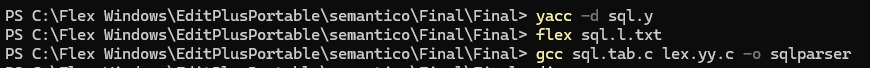
\includegraphics[scale=0.8]{compilacion.jpeg}
        \caption{Generación del archivo ejecutable}
        \label{fig:ejecutablesql}
    \end{figure}

\end{enumerate}

\newpage

\subsection{Pruebas y resultados}

Las pruebas realizadas consistieron en ingresar diferentes instrucciones SQL desde la consola para verificar el correcto funcionamiento del analizador sintáctico. \\

Se evaluaron tanto casos válidos como inválidos para comprobar la capacidad del sistema de detectar errores sintácticos y aceptar consultas correctamente estructuradas.

Entre las pruebas realizadas se incluyeron:

\begin{itemize}
    \item Consultas \texttt{SELECT} con cláusulas \texttt{FROM} y \texttt{WHERE}.
    \item Inserciones mediante \texttt{INSERT INTO}.
    \item Actualizaciones usando \texttt{UPDATE SET}.
    \item Eliminaciones con \texttt{DELETE FROM}.
\end{itemize}

A continuación se muestran algunos ejemplos de casos aceptados y rechazados por el analizador.

\begin{figure}[h]
    \centering
   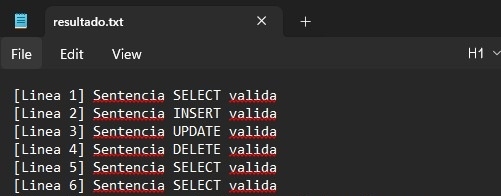
\includegraphics[scale=0.8]{aceptacion.jpeg}
    \caption{Casos de aceptación}
    \label{fig:aceptacion}
\end{figure}

\begin{figure}[h]
    \centering
   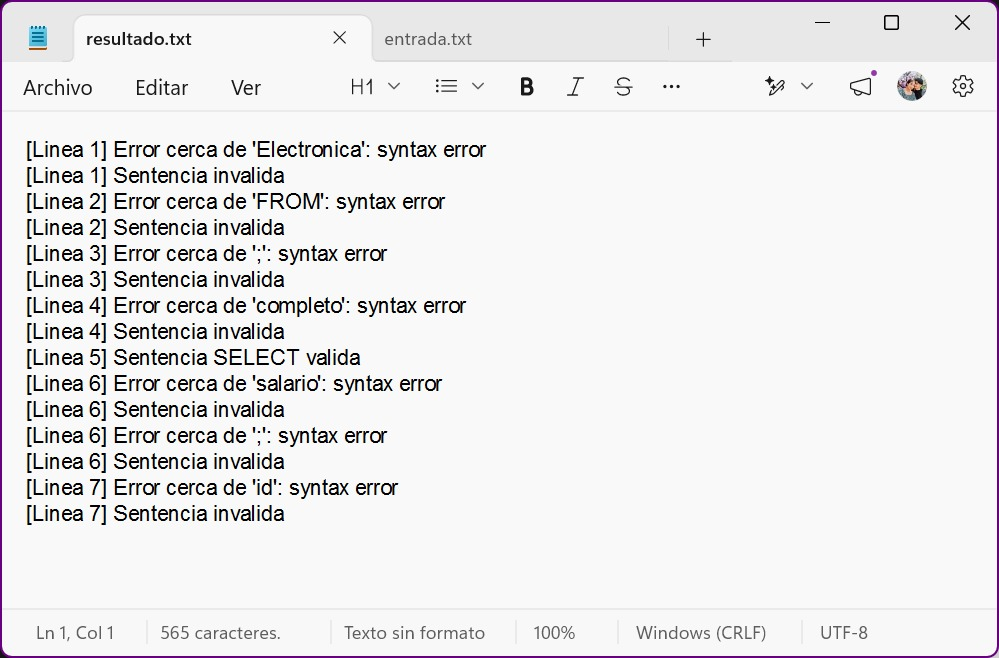
\includegraphics[scale=0.3]{error.jpeg}
    \caption{Casos de rechazo}
    \label{fig:rechazo}
\end{figure}

\newpage

\section{5.Cuestionario}

\begin{enumerate}
    \item \textbf{¿Cómo se describe la sintaxis de un lenguaje de programación mediante gramáticas (en notación 
BNF), y qué ventajas ofrecen estas herramientas en el diseño de compiladores?}\\

La sintaxis es descrita mediante reglas de producción en BNF que define cómo se construyen las expresiones válidas del lenguaje. Estas gramáticas son las que facilitan el diseño de compiladores, la detección de errores y la generación automática de analizadores sintácticos.

\item \textbf{¿Qué roles desempeñan Lex y Yacc en el análisis léxico y sintáctico, y cómo se complementan en el 
desarrollo de un compilador?}\\

Son lenguajes de programacion que facilitan la creacion de tokens y arboles semanticos, para la nueva creacion de compiladores 

\item \textbf{Al implementar un analizador léxico en Lex, ¿qué patrones se deben definir para identificar 
correctamente los tokens de números y operadores aritméticos?}\\

Se deben definir las expresiones regulares correctamente para reconocer números enteros o decimales, y tambien los operadores como suma, resta, multiplicación y división.

\item \textbf{Durante la validación de una línea de código como 133 * 25, ¿cómo identifica errores sintácticos el 
programa en Yacc y qué estrategias utiliza para recuperarse de ellos?}\\

Yacc compara la secuencia de tokens con las reglas de la gramática. Si este encuentra una estructura inválida, procede a generar un mensaje de error y el mismo utiliza reglas de recuperación para continuar el análisis.

\end{enumerate}

\section{6. Conclusiones}
   A lo largo del desarrollo de nuestra practica se puso en practica todos los conocimientos que se han adquirido a lo largo del semestre que hemos necesitado del analizador lexico para poner en practica el analisis sintactico. Con esto al momento de compilar pudimos resolver los errores que se tenian debido a la sintaxis diferentes \\
   Al final, se logro comprender el funcionamiento de ambos analisis (lexico y sintactico) y como se relacionan entre si, ademas de que se comprobo como se necesitan y se relacionan el uno del otro para poder funcionar de manera correcta.
   
    \newpage
    
\section{Referencias Bibliográficas}
    %Formato APA 7° Ed.
    \begin{thebibliography}{100}
        \bibitem{compiladores1}d
Aho, A. V., Ravi, S. A. V. \& Ullman, J. D. ({\bf 1998}). Compiladores: Principios, técnicas y herramientas. Addison Wesley Longman. México. 

\bibitem{compiladores2}
Giró, J., Vázquez, J., Meloni, B., Constable, L. ({\bf 2015}). Lenguajes formales y teoría 
de automátas. Editorial Alfaomega. Argentina.

    \end{thebibliography}

 
        

\end{document}

